\documentclass[conference]{IEEEtran}
\IEEEoverridecommandlockouts
% Template-aligned conference preamble
\usepackage{cite}
\usepackage{amsmath,amssymb,amsfonts}
\interdisplaylinepenalty=2500
\usepackage{algorithmic}
\usepackage{algorithm}
\usepackage{graphicx}
\usepackage{textcomp}
\usepackage{xcolor}
\def\BibTeX{{\rm B\kern-.05em{\sc i\kern-.025em b}\kern-.08em
    T\kern-.1667em\lower.7ex\hbox{E}\kern-.125emX}}
\begin{document}
\title{Smart Parking Allocation \& Cruising Reduction System Based on Real-Time Reservation Database}

\author{
    \IEEEauthorblockN{1\textsuperscript{st} Haonan Cheng}
    \IEEEauthorblockA{\textit{Dept. of CST} \\
        \textit{Graduate School of ICT, Ajou University}\\
        Suwon, South Korea \\
        haonan.cheng@hotmail.com}
    \and
    \IEEEauthorblockN{2\textsuperscript{nd} Mingyuan Zhou}
    \IEEEauthorblockA{\textit{Dept. of CST} \\
        \textit{Graduate School of ICT, Ajou University}\\
        Suwon, South Korea \\
        ruyezhou020726@gmail.com}
}

\maketitle

\begin{abstract}
Urban traffic congestion is significantly exacerbated by vehicles cruising for parking, which wastes fuel, increases emissions, and reduces overall network efficiency. This paper presents a smart parking allocation and cruising reduction system built on SUMO, Python TraCI, and PostgreSQL. The controller keeps reservation state in Python dictionaries, synchronizes parking inventory and run summaries to relational tables, and applies a tiered pricing policy when local occupancy exceeds 70\% and 90\%. In the database-backed evaluation, Scenario A parks 2,498 of 2,500 planned vehicles by the 7,200~s simulation limit, whereas Scenario B parks all 2,500 vehicles by 3,922~s while also reducing average search time, fuel consumption, and selected emission indicators.
\end{abstract}

\begin{IEEEkeywords}
    Smart Parking, Cruising for Parking, Microscopic Traffic Simulation, SUMO, Relational Database, Dynamic Pricing, Python TraCI, PostgreSQL.
\end{IEEEkeywords}

\section{Introduction}
As urbanization accelerates globally, urban mobility faces unprecedented challenges. A pervasive contributor to traffic congestion is ``cruising for parking'' \cite{b1}. In Central Business Districts (CBDs), cruising vehicles can account for 20\% to 30\% of total traffic volume during peak hours \cite{b2}.

Traditional parking management relies on static signage or localized IoT sensor networks \cite{b3}. While providing real-time status, they lack active system-wide coordination. When multiple vehicles simultaneously target a single available spot, localized bottlenecks emerge, forcing unsuccessful drivers to resume cruising.

To resolve this, modern Intelligent Transportation Systems (ITS) must shift from ``reactive searching'' to ``proactive reservation'' \cite{b4}. However, simulating and implementing such a system at a microscopic level presents massive computational challenges. This paper bridges the gap between microscopic traffic simulation and enterprise-grade databases. Our core contributions include:

\begin{enumerate}
    \item \textbf{Mathematical Formulation}: Modeling parking allocation as a multi-objective optimization problem balancing distance, cost, and network load.
    \item \textbf{High-Performance Reservation State}: Using Python dictionaries inside the TraCI control loop to handle high-frequency reservation queries, with batched PostgreSQL updates to preserve persistent scenario logs without slowing the simulation.
    \item \textbf{Multi-Tier Dynamic Pricing}: Implementing a demand-responsive algorithm that raises base prices by 1.5x and 2.0x at 70\% and 90\% occupancy, redirecting traffic to peripheral lots organically.
    \item \textbf{Microscopic Evaluation}: Utilizing the TraCI interface to simulate 2,500 planned trips, quantifying completion time, search time, fuel consumption, explicit cruising distance, selected emission metrics, and network speed using the same monitoring pipeline used during execution.
\end{enumerate}

\section{Related Work}

\subsection{Modeling and Impacts of Cruising}
Shoup \cite{b1} and Inci \cite{b2} documented the economic and environmental ramifications of underpriced parking. However, macroscopic models often fail to capture the complex, agent-level interactions occurring at intersections and parking lot entrances \cite{b5}.

\subsection{Smart Parking and IoT Integration}
Lin et al. \cite{b3} surveyed sensor-based parking systems. Geng and Cassandras \cite{b4} proposed resource allocation and reservation systems. Yet, many conceptual proposals rely on discrete-event simulators rather than high-fidelity microscopic environments.

\subsection{Dynamic Pricing in Transportation}
Dynamic pricing effectively manages peak demand in ride-sharing and tolling. Fosgerau \cite{b6} and Pierce \cite{b7} analyzed utilization-based parking fee optimization. We embed a multi-tier pricing logic directly into the simulation loop to observe the immediate microscopic impacts on vehicle routing.

\subsection{Data Synchronization in Co-Simulations}
Wegener et al. \cite{b8} discussed TraCI latency bottlenecks when scaling up to thousands of vehicles. In this project, the TraCI control loop keeps the active reservation state in Python dictionaries and writes durable updates to PostgreSQL at fixed simulation intervals.

\section{System Architecture and Methodology}
The architecture forms a closed-loop system between the SUMO simulation, the Python TraCI controller, and the PostgreSQL database.

\begin{figure}[htbp]
    \centering
    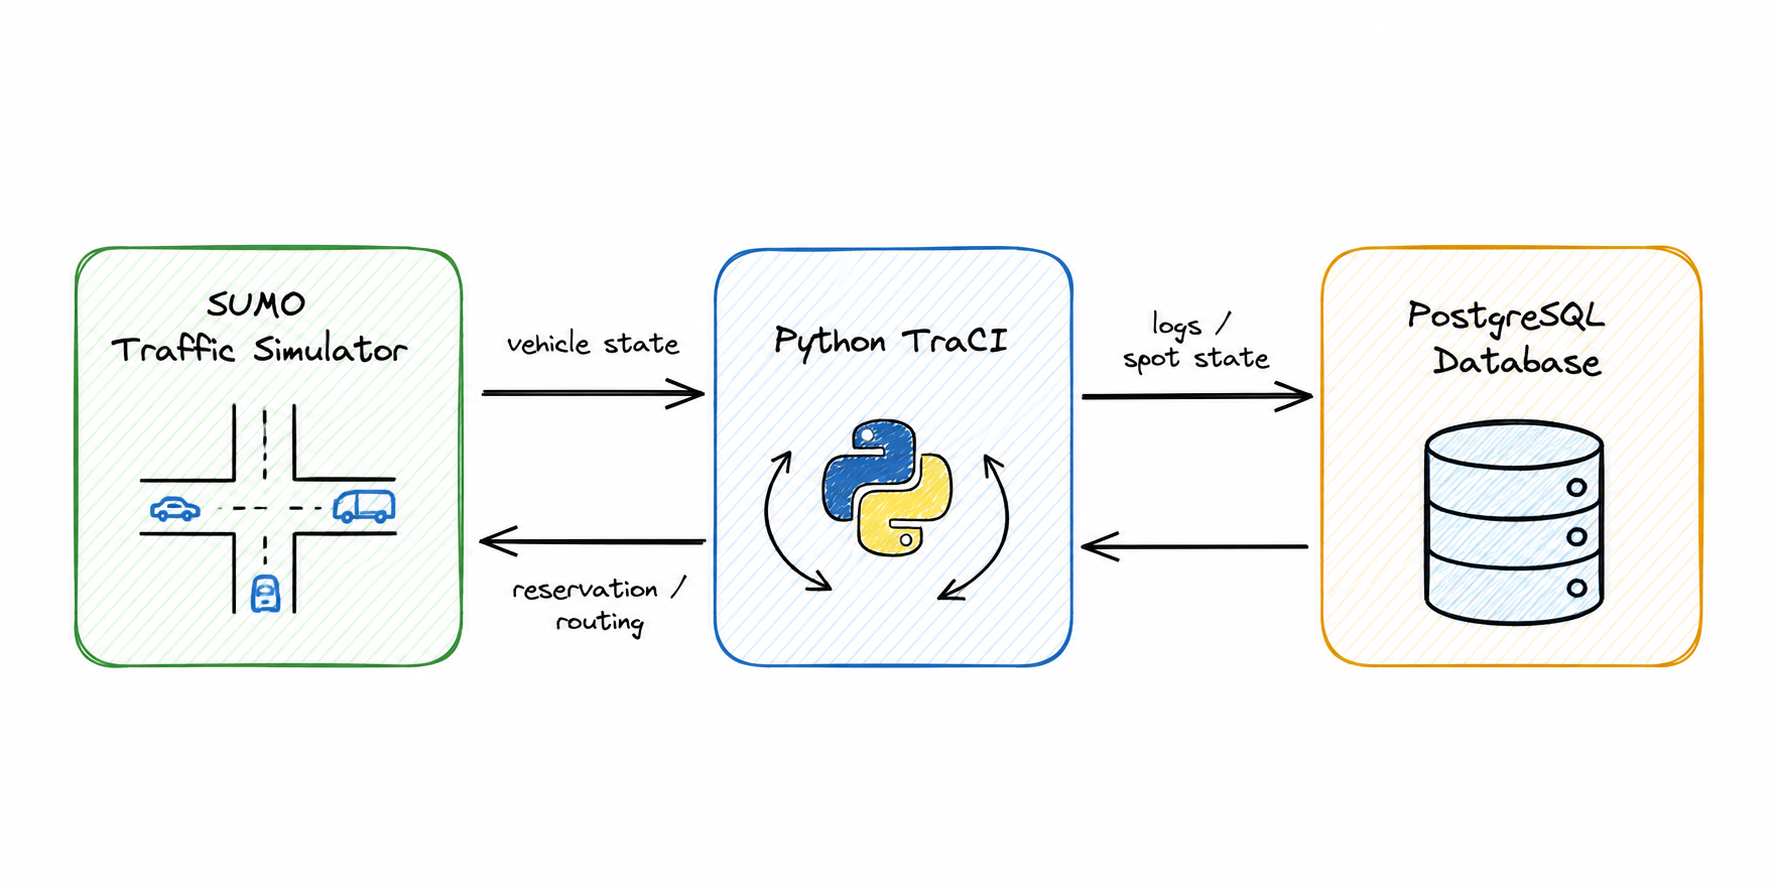
\includegraphics[width=\linewidth]{paper_assets/fig1_architecture_gpt.png}
    \caption{System architecture showing the data flow between SUMO, Python TraCI, and PostgreSQL.}
    \label{fig:architecture}
\end{figure}

\subsection{Problem Formulation}
The objective is to assign an optimal parking spot $p_j \in P$ to a vehicle $v_i \in V$, minimizing the generalized parking cost. The assignment logic executes as follows:

\begin{enumerate}
    \item \textbf{Candidate Spot Filtering (Capacity Constraint)}:
          The system iterates through the reservation-state dictionary, including a spot in the candidate list only if its booked capacity is strictly less than its total capacity:
          \begin{equation}
              \sum_{i \in V} x_{ij} < Capacity(p_j), \quad \forall p_j \in P
          \end{equation}

    \item \textbf{Dynamic Price Calculation}:
          For each available spot, the real-time occupancy rate $\rho$ is retrieved. The current price $Price(p_j)$ is adjusted based on the 70\% and 90\% occupancy thresholds.

    \item \textbf{Cost Evaluation (Cost Function)}:
          The generalized cost $C_{ij}$ to park at candidate spot $p_j$ is calculated based on the vehicle's current position:
          \begin{equation}
              C_{ij} = Price(p_j) + d_{route}(v_i, p_j) \cdot c_d
          \end{equation}
          Where $d_{route}$ is the estimated route distance from the vehicle to the parking area and $c_d$ is the per-meter monetary distance cost. The implementation sets $c_d=0.0025$, so 1 km of additional driving is evaluated as 2.5 currency units.

    \item \textbf{Greedy Assignment}:
          The system extracts the candidate spot that yields the minimum $C_{ij}$, transforming an expensive global optimization problem into an efficient, low-latency local assignment for each vehicle.
\end{enumerate}

\subsection{Database and State Dictionary Mechanism}
The system utilizes a streamlined PostgreSQL schema to minimize transaction overhead while preserving the fields needed for reproducible comparison:

\begin{itemize}
    \item \textbf{\texttt{parking\_spots}}: Stores the parking inventory and the dynamic reservation state used by the controller.
          \begin{itemize}
              \item \textit{Static}: \texttt{spot\_id}, \texttt{edge\_id}, \texttt{spot\_type}, \texttt{capacity}, and \texttt{base\_price}.
              \item \textit{Dynamic}: \texttt{occupied} and \texttt{current\_price}, synchronized from the Python state dictionary.
          \end{itemize}
    \item \textbf{\texttt{cruising\_logs}}: Tracks vehicle-level parking behavior, travel effort, and environmental outputs.
          \begin{itemize}
              \item \textit{Core}: \texttt{log\_id}, \texttt{vehicle\_id}, \texttt{scenario}, and \texttt{final\_spot\_id}.
              \item \textit{Operation}: \texttt{search\_time\_sec}, \texttt{cruising\_distance\_m}, and \texttt{total\_fuel\_mg}.
              \item \textit{Environment}: \texttt{total\_co2\_mg}, \texttt{total\_nox\_mg}, and \texttt{total\_pmx\_mg}.
          \end{itemize}
    \item \textbf{\texttt{simulation\_runs}}: Stores run-level outcomes, including \texttt{completion\_time\_sec}, \texttt{total\_vehicles}, \texttt{parked\_vehicles}, \texttt{failed\_vehicles}, and \texttt{parking\_rate}.
\end{itemize}

\textbf{Dictionary-based Reservation Workflow:}
\begin{enumerate}
    \item \textbf{Initialization}: Before the simulation begins, the \texttt{parking\_spots} table is loaded into a Python dictionary.
    \item \textbf{Simulation Loop}: The reservation engine executes $O(1)$ lookups within the dictionary, updating occupancy rates and calculating prices instantly in memory.
    \item \textbf{Batch Synchronization}: Every 60 simulation seconds, the Python TraCI controller writes a bulk \texttt{UPDATE} transaction to PostgreSQL through \texttt{sync\_spots} or \texttt{sync\_spots\_priced}.
\end{enumerate}

\begin{algorithm}[htbp]
    \caption{Dynamic Pricing \& Reservation Engine}
    \label{alg:reservation}
    \begin{algorithmic}[1]
        \REQUIRE Vehicle $v_i$, State Dictionary $\mathcal{D}$
        \ENSURE Optimal Parking Spot $p_{opt}$
        \STATE $min\_cost \gets \infty$
        \STATE $p_{opt} \gets \text{NULL}$
        \FOR{\textbf{each} spot $p_j \in \mathcal{D}$}
        \IF{$p_j.\text{booked} < p_j.\text{capacity}$}
        \STATE $\rho \gets p_j.\text{booked} / p_j.\text{capacity}$
        \IF{$\rho > 0.90$}
        \STATE $P_{current} \gets p_j.\text{base\_price} \times 2.0$
        \ELSIF{$\rho > 0.70$}
        \STATE $P_{current} \gets p_j.\text{base\_price} \times 1.5$
        \ELSE
        \STATE $P_{current} \gets p_j.\text{base\_price}$
        \ENDIF
        \STATE $dist \gets \text{LocalGraphRouteDistance}(v_i, p_j)$
        \STATE $cost \gets P_{current} + (dist \times UNIT\_DIST\_COST)$
        \IF{$cost < min\_cost$}
        \STATE $min\_cost \gets cost$
        \STATE $p_{opt} \gets p_j$
        \ENDIF
        \ENDIF
        \ENDFOR
        \IF{$p_{opt} \neq \text{NULL}$}
        \STATE $p_{opt}.\text{booked} \gets p_{opt}.\text{booked} + 1$
        \STATE \text{Route vehicle} $v_i$ \text{to} $p_{opt}$ \text{via TraCI}
        \ENDIF
        \RETURN $p_{opt}$
    \end{algorithmic}
\end{algorithm}

\subsection{Multi-Tier Dynamic Pricing Logic}
As detailed in Algorithm \ref{alg:reservation}, the current price $P_{current}$ is a piecewise function dependent on the real-time local occupancy rate $\rho$:
\begin{equation}
    P_{current} =
    \begin{cases}
        P_{base},            & \text{if } \rho \le 0.70        \\
        1.5 \times P_{base}, & \text{if } 0.70 < \rho \le 0.90 \\
        2.0 \times P_{base}, & \text{if } \rho > 0.90
    \end{cases}
\end{equation}

The implemented Scenario B script evaluates this function at every simulation step before handling newly departed vehicles. Small on-street records are aggregated at street level using \texttt{STREET\_SPOT\_THRESHOLD=3}; large off-street hubs are priced by their own booked-capacity ratio. Vehicle-to-spot distance is estimated in Python from a cached SUMO network graph using one Dijkstra search per newly departed vehicle, and the cost function uses \texttt{UNIT\_DIST\_COST=0.0025} to convert route distance into the same monetary unit as parking price.

\subsection{Cruising Detection and TraCI Integration}
In the baseline scenario, vehicles navigate blindly and search from the road network itself. The baseline script builds opposite-edge and outgoing-edge maps from \texttt{demo.net.xml}, scans visible parking areas within a 180 m sight distance, checks intersections every three simulation steps, and reroutes a vehicle when the remaining route is nearly exhausted. A locked target is abandoned after 120 seconds if the vehicle cannot park there, reproducing the unstable behavior of competitive curbside search.

Scenario B removes this street-scanning loop. Each departed vehicle is assigned once through the in-memory dictionary, routed to the chosen parking area with TraCI, and settled when \texttt{traci.vehicle.isStoppedParking} becomes true. The log row for Scenario B therefore records zero explicit cruising distance for the reservation phase; fuel and emission values reflect the normal drive from origin to the assigned parking facility.

\section{Experimental Setup}
The evaluation was conducted using SUMO (version 1.26.0).

\subsection{Network Topology and Capacity}
The simulated network is generated by the project script \texttt{generate\_network.ps1}. It creates a 15 $\times$ 15 grid with 225 non-internal junctions, 840 bidirectional road edges, and 2,520 lanes. Each grid segment is 200 m, each edge has three lanes, the default speed is 11.11 m/s, and SUMO is asked to infer actuated traffic signals.

The parking inventory is generated by \texttt{generate\_parking.py} and materialized in both \texttt{schema.sql} and \texttt{parking.add.xml}. The database contains 850 parking records, but the physical capacity is 2,700 spaces: 800 one-space on-street records and 50 off-street hubs with 38 spaces each. This distinction matters because the reservation system reasons over database records while SUMO stops vehicles at the corresponding parking-area objects.

Figures \ref{fig:network_overview}--\ref{fig:offstreet_detail} provide the spatial context used by both scenario scripts: the complete grid, an intersection-level detail view, and an off-street parking facility.

\begin{figure}[!t]
    \centering
    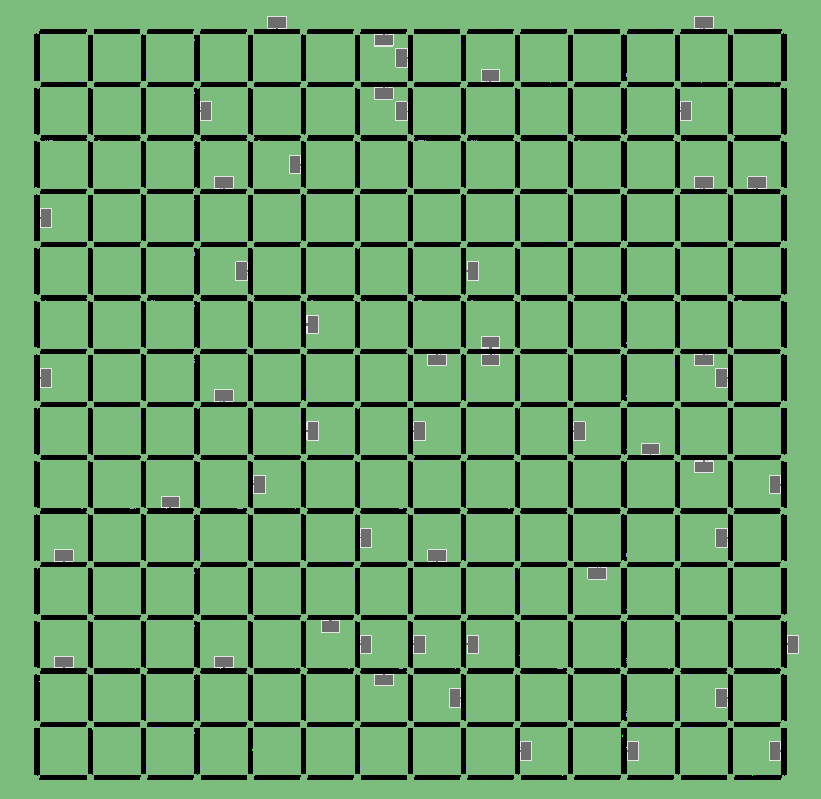
\includegraphics[width=\linewidth]{paper_assets/network_overview.png}
    \caption{Overall SUMO road network with generated parking facilities.}
    \label{fig:network_overview}
\end{figure}

\begin{figure}[!t]
    \centering
    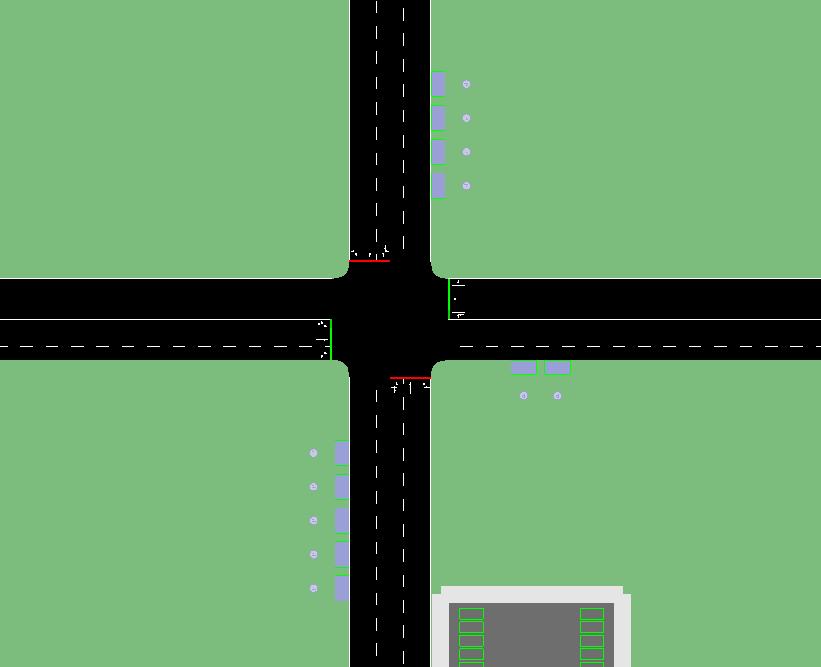
\includegraphics[width=\linewidth]{paper_assets/intersection_detail.png}
    \caption{Intersection-level detail of the generated grid network.}
    \label{fig:intersection_detail}
\end{figure}

\begin{figure}[!t]
    \centering
    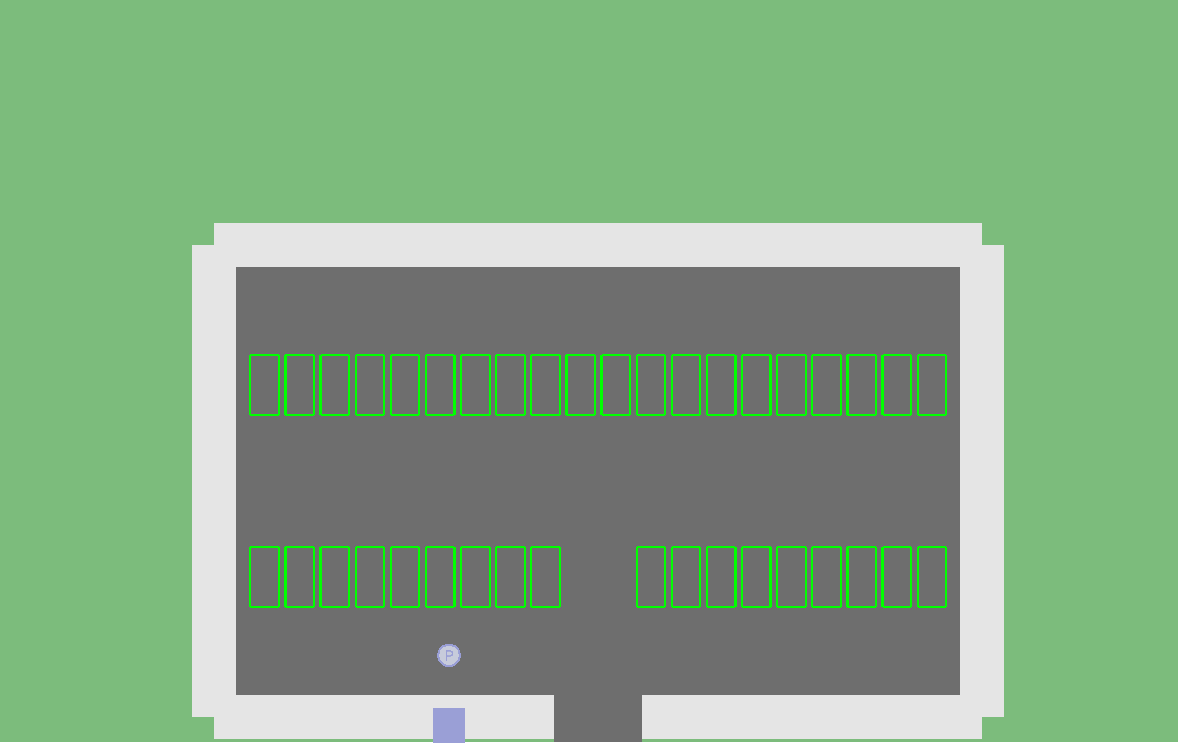
\includegraphics[width=\linewidth]{paper_assets/offstreet_parking_detail.png}
    \caption{Off-street parking facility represented in the generated parking inventory.}
    \label{fig:offstreet_detail}
\end{figure}

\subsection{Simulation Parameters}
\begin{table}[htbp]
    \caption{Simulation Configuration Parameters}
    \label{tab:parameters}
    \centering
    \footnotesize
    \begin{tabular}{|p{0.41\linewidth}|p{0.43\linewidth}|}
        \hline
        \textbf{Parameter} & \textbf{Configuration Value} \\
        \hline
        Simulator & Eclipse SUMO \\
        Car-Following Model & Krauss \cite{b10} \\
        Total Vehicles & 2,500 \\
        Simulation Duration & 7,200 seconds (2 hours) \\
        Trip Departures & 3.0--3,599.8 seconds in \texttt{demo.trips.xml} \\
        Parking Records & 850 (800 on-street, 50 off-street hubs) \\
        Physical Parking Capacity & 2,700 spaces \\
        Database Backend & PostgreSQL 18.4 \\
        Control Interface & TraCI via Python 3.10 \\
        Pricing Thresholds ($\rho$) & Tier 1: 70\% (1.5x), Tier 2: 90\% (2.0x) \\
        \hline
    \end{tabular}
\end{table}

\begin{table}[htbp]
    \caption{Project Constants Used by the Two Scenario Scripts}
    \label{tab:implementation_constants}
    \centering
    \footnotesize
    \begin{tabular}{|p{0.43\linewidth}|p{0.41\linewidth}|}
        \hline
        \textbf{Implementation Setting} & \textbf{Value in Project Code} \\
        \hline
        Baseline sight distance & 180 m \\
        Baseline parking scan interval & 3 simulation steps \\
        Target waiting timeout & 120 seconds \\
        Database sync interval & 60 seconds \\
        Smart distance cost & $0.0025$ currency units per meter \\
        Street aggregation threshold & capacity $\leq 3$ spaces \\
        Monitoring refresh interval & 5 simulation steps \\
        \hline
    \end{tabular}
\end{table}

\subsection{Evaluation Scenarios}
\begin{itemize}
    \item \textbf{Scenario A (Baseline Random Search)}: The Smart Allocation system is deactivated. Drivers search from the roadway, scan nearby curbside spaces, create pending targets, abandon unavailable spots, and randomly reroute when a route segment is exhausted.
    \item \textbf{Scenario B (Smart Allocation)}: The reservation architecture is active. Vehicles query the state dictionary when they depart, receive a unified-cost-minimizing spot, increment the booked count, and synchronize occupancy and price to PostgreSQL in batches.
\end{itemize}

\section{Results and Performance Evaluation}

Figure \ref{fig:scenario_a_monitor} shows the baseline monitor. The six-panel layout includes active searching vehicles, cumulative parked vehicles, explicit cruising distance, average parking search time, cumulative fuel, and network average speed. The curve reaches the two-hour boundary rather than a clean all-parked completion: the database log records 2,498 parked vehicles out of 2,500 planned trips, a 99.92\% parking rate, with 2,692.06 km of explicit cruising and 371.29 s of average search time.

\begin{figure}[!t]
    \centering
    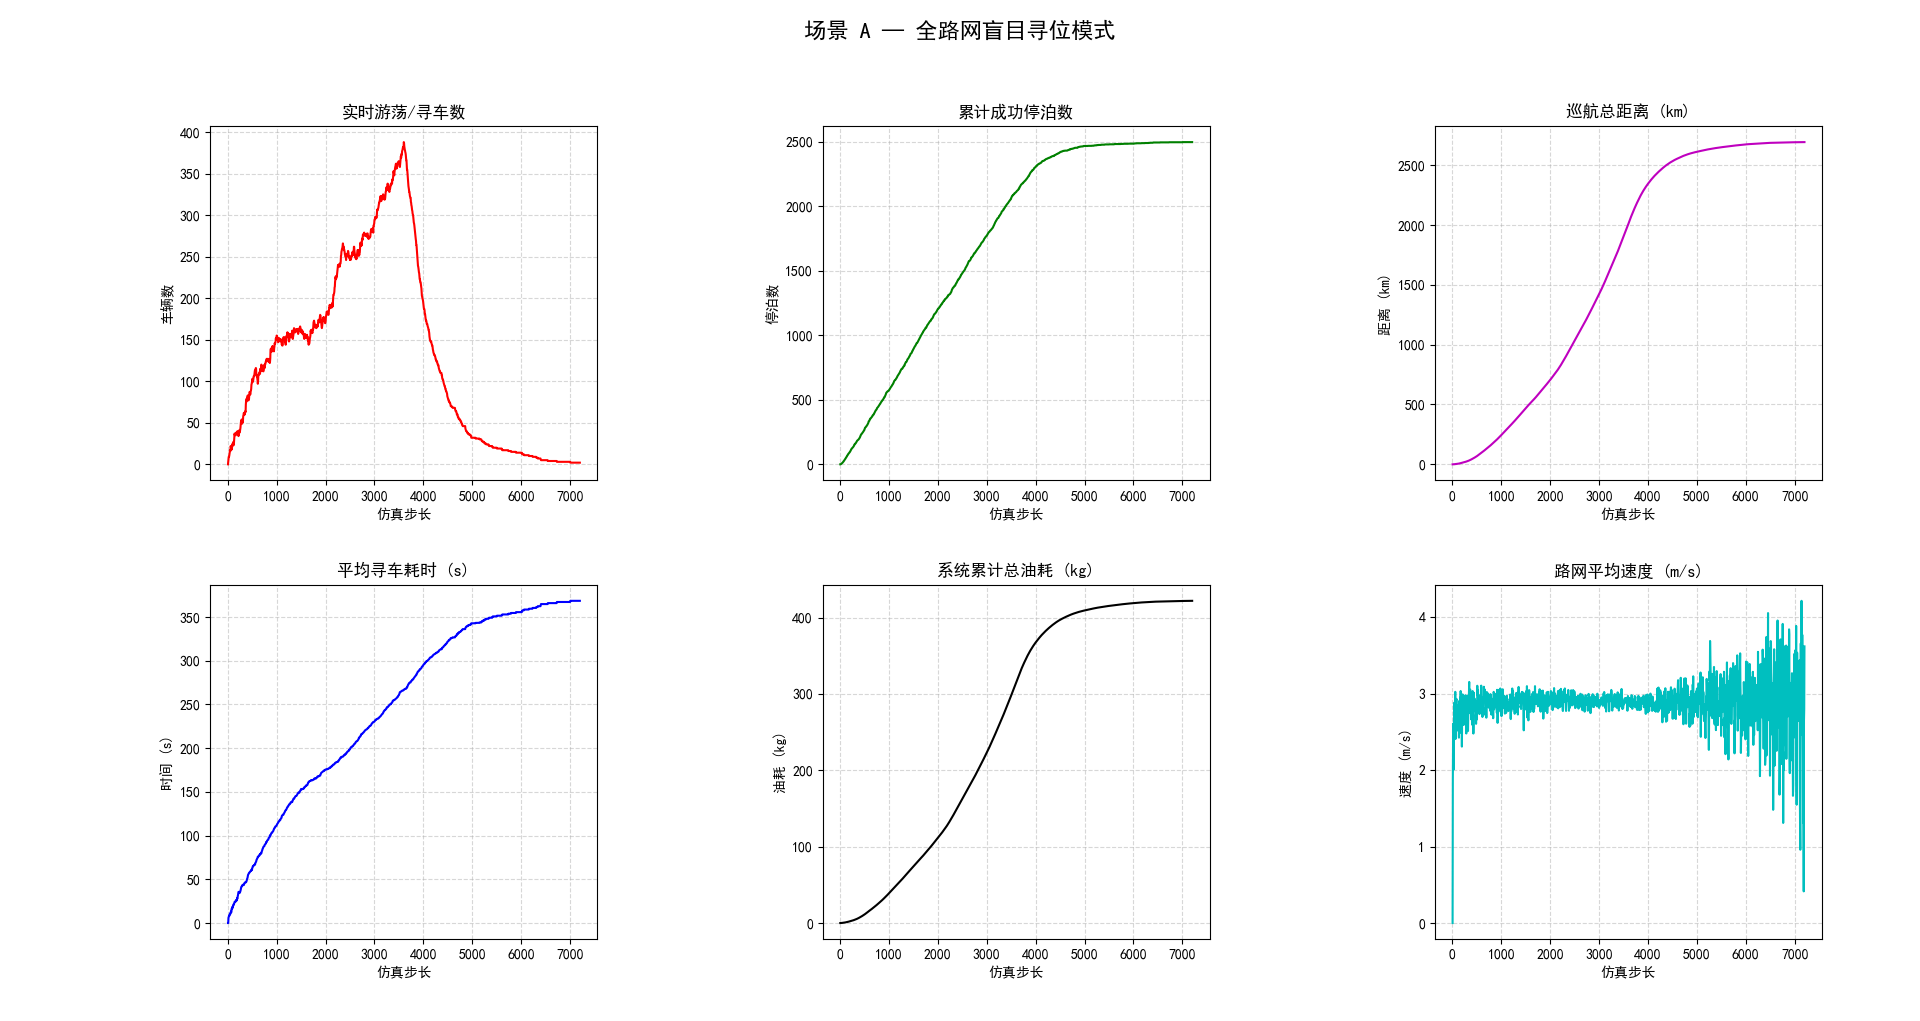
\includegraphics[width=\linewidth]{paper_assets/scenario_A_monitor.png}
    \caption{Scenario A monitoring panel generated by the project Matplotlib monitor: blind network-wide search with active searchers, cumulative parked vehicles, cruising distance, average search time, cumulative fuel, and network speed.}
    \label{fig:scenario_a_monitor}
\end{figure}

Figure \ref{fig:scenario_b_monitor} shows the smart reservation monitor. Its four-panel layout focuses on cumulative successful parking, average search time, cumulative fuel, and network average speed. Scenario B reaches all 2,500 parked vehicles at 3,922 s, maintains a 100.00\% parking rate, and records a database average search time of 108.72 s.

\begin{figure}[!t]
    \centering
    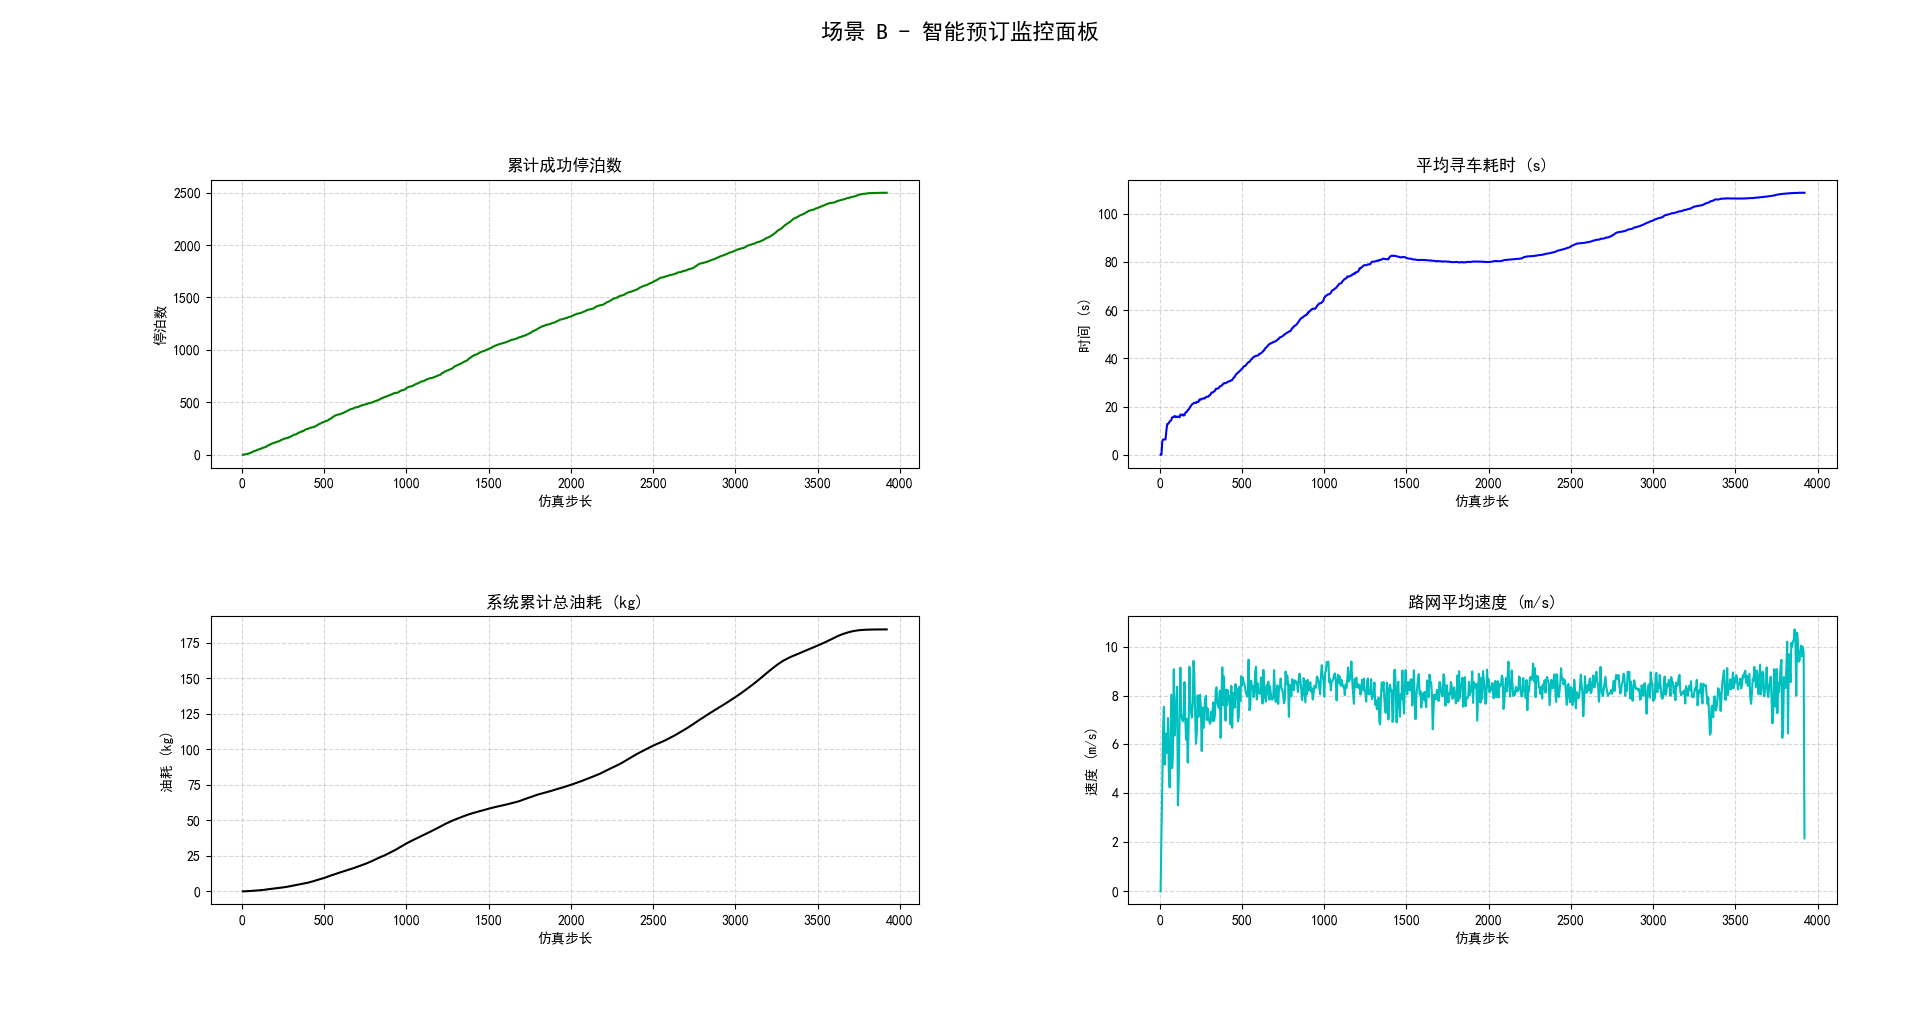
\includegraphics[width=\linewidth]{paper_assets/scenario_B_monitor.png}
    \caption{Scenario B monitoring panel generated by the project Matplotlib monitor: smart reservation with cumulative parked vehicles, average search time, cumulative fuel, and network speed.}
    \label{fig:scenario_b_monitor}
\end{figure}

The evaluation uses two database sources. The \texttt{simulation\_runs} table records the simulation ending time, while \texttt{Cruising\_Logs} aggregates vehicle-level parking outcomes, travel effort, fuel, and selected emission indicators including CO$_2$, NOx, and PMx. Parking rate is calculated from vehicle-level parking records, so Scenario A is reported as 2,498 parked vehicles out of 2,500 planned trips. The key operational result remains total simulation time: Scenario B reaches all-vehicle completion in 3,922 s, whereas Scenario A reaches the two-hour 7,200 s simulation limit with two vehicles unresolved in the vehicle log.

\begin{table}[htbp]
    \caption{Parking Rate and Simulation Ending Time}
    \label{tab:run_metrics}
    \centering
    \footnotesize
    \begin{tabular}{|p{0.37\linewidth}|c|c|}
        \hline
        \textbf{Metric} & \textbf{Scenario A} & \textbf{Scenario B} \\
        \hline
        Planned vehicles & 2,500 & 2,500 \\
        Parked vehicles & 2,498 & \textbf{2,500} \\
        Unparked vehicles & 2 & \textbf{0} \\
        Parking rate & 99.92\% & \textbf{100.00\%} \\
        Ending time (s) & 7,200 & \textbf{3,922} \\
        Ending time (min) & 120.00 & \textbf{65.37} \\
        Ending condition & Time limit & All parked \\
        \hline
    \end{tabular}
\end{table}

\begin{table}[htbp]
    \caption{Operational and Selected Environmental Aggregates}
    \label{tab:vehicle_metrics}
    \centering
    \footnotesize
    \begin{tabular}{|p{0.37\linewidth}|c|c|}
        \hline
        \textbf{Metric} & \textbf{Scenario A} & \textbf{Scenario B} \\
        \hline
        Avg. search time (s) & 371.29 & \textbf{108.72} \\
        Explicit cruising (km) & 2,692.06 & \textbf{0.00} \\
        Total fuel (kg) & 421.87 & \textbf{184.58} \\
        Total CO$_2$ (kg) & 1,301.31 & \textbf{569.37} \\
        Total NOx (g) & 413.17 & \textbf{190.02} \\
        Total PMx (g) & 46.53 & \textbf{46.08} \\
        \hline
    \end{tabular}
\end{table}

Relative to the baseline, smart allocation shortens the simulation ending time by 3,278 s, or 45.53\%, while also improving the parking rate from 99.92\% to 100.00\%. Vehicle-level logs show a 70.72\% lower average search time, elimination of explicit cruising during the reservation phase, 56.25\% lower fuel consumption, 56.25\% lower CO$_2$, 54.01\% lower NOx, and 0.97\% lower PMx.

\section{Conclusion}
This paper presented a Smart Parking Allocation system designed to reduce the ``cruising for parking'' phenomenon. The Python TraCI control loop coordinates SUMO vehicle routing with PostgreSQL-backed scenario logging, real-time reservation state updates, and dashboard-level comparison of two executable SUMO scenarios. In the database results, Scenario A parks 2,498 of 2,500 planned vehicles by the 7,200 s simulation limit, while Scenario B parks all 2,500 vehicles by 3,922 s. Scenario B therefore improves both parking completion and total simulation time, while also reducing average search time by 70.72\%, fuel and CO$_2$ by 56.25\%, NOx by 54.01\%, and PMx by 0.97\%.

\begin{thebibliography}{00}
    \bibitem{b1} D. C. Shoup, ``Cruising for parking,'' \textit{Transport Policy}, vol. 13, no. 6, pp. 479--486, 2006.
    \bibitem{b2} E. Inci, ``A review of the economics of parking,'' \textit{Economics of Transportation}, vol. 4, no. 1-2, pp. 50--63, 2015.
    \bibitem{b3} T. Lin, H. Rivano, and F. Le Mouel, ``A Survey of Smart Parking Solutions,'' \textit{IEEE Transactions on Intelligent Transportation Systems}, vol. 18, no. 12, pp. 3229--3253, Dec. 2017.
    \bibitem{b4} Y. Geng and C. G. Cassandras, ``New smart parking system based on resource allocation and reservations,'' \textit{IEEE Transactions on Intelligent Transportation Systems}, vol. 14, no. 3, pp. 1129--1139, 2013.
    \bibitem{b5} R. Arnott and J. Rowse, ``Modeling parking,'' \textit{Journal of Urban Economics}, vol. 45, no. 1, pp. 97--124, 1999.
    \bibitem{b6} M. Fosgerau and A. de Palma, ``The dynamics of urban traffic congestion and the price of parking,'' \textit{Journal of Public Economics}, vol. 105, pp. 106--115, 2013.
    \bibitem{b7} G. Pierce and D. Shoup, ``Getting the prices right: An evaluation of pricing parking by demand in San Francisco,'' \textit{Journal of the American Planning Association}, vol. 79, no. 1, pp. 67--81, 2013.
    \bibitem{b8} A. Wegener, M. Piórkowski, M. Raya, H. Hellbrück, S. Fischer, and J.-P. Hubaux, ``TraCI: an interface for coupling road traffic and network simulators,'' \textit{Proceedings of the 11th Communications and Networking Simulation Symposium}, 2008, pp. 155--163.
    \bibitem{b10} S. Krauss, ``Microscopic modeling of traffic flow: Investigation of collision free vehicle dynamics,'' Ph.D. dissertation, DLR, Cologne, Germany, 1998.
    \bibitem{b11} M. Behrisch, L. Bieker, J. Erdmann, and D. Krajzewicz, ``SUMO Simulation of Urban Mobility: An Overview,'' \textit{Proceedings of SIMUL 2011, The Third International Conference on Advances in System Simulation}, 2011.
\end{thebibliography}

\end{document}




